\documentclass[11pt,a4paper]{article}

% ---------------------------------------------------------------------------
% Packages
% ---------------------------------------------------------------------------
\usepackage[utf8]{inputenc}
\usepackage[T1]{fontenc}
\usepackage{lmodern}
\usepackage[margin=2.5cm]{geometry}
\usepackage{amsmath,amssymb,amsthm,bm}
\usepackage{graphicx}
\usepackage{booktabs}
\usepackage{tabularx}
\usepackage{multirow}
\usepackage{subcaption}
\usepackage{xcolor}
\usepackage{tikz}
\usetikzlibrary{arrows.meta,positioning,shapes.geometric,fit,calc,automata}
\usepackage{algorithm}
\usepackage{algpseudocode}
\usepackage{enumitem}
\usepackage{microtype}
\usepackage[numbers,sort&compress]{natbib}
\usepackage[hidelinks]{hyperref}
\usepackage{cleveref}

\graphicspath{{figures/}}

\theoremstyle{definition}
\newtheorem{definition}{Definition}
\newtheorem{assumption}{Assumption}
\newtheorem{hypothesis}{Hypothesis}
\newtheorem{resq}{Research Question}
\crefname{hypothesis}{Hypothesis}{Hypotheses}
\crefname{resq}{RQ}{RQs}

\newcommand{\obs}{\bm{o}}
\newcommand{\act}{\bm{a}}
\newcommand{\state}{\bm{q}}
\newcommand{\img}{\bm{I}}
\newcommand{\depthmap}{\bm{D}}
\newcommand{\pol}{\pi_\theta}
\newcommand{\ctrl}{c_\psi}
\newcommand{\gate}{g}
\newcommand{\E}{\mathbb{E}}
\newcommand{\R}{\mathbb{R}}
\newcommand{\ind}{\mathbb{1}}
\newcommand{\todo}[1]{\textcolor{red}{[#1]}}

\title{\vspace{-1.2cm}
Metric Wrist Depth as a Contact Proxy\\
for Imitation-Learned Grasping on Force-Blind Low-Cost Manipulators\\[0.4em]
{\large A research programme in machine learning for visuomotor control}}
\author{Romil Modi\\
\small SO-101 Visuomotor Manipulation Platform\\
\small\url{https://github.com/romil0001/SO101_Visuomotor_Manipulation}}
\date{October 2026 \quad\textperiodcentered\quad Research proposal, version 1}

\begin{document}
\maketitle

% ---------------------------------------------------------------------------
\begin{abstract}
Imitation-learned visuomotor policies on low-cost, position-controlled robot arms fail overwhelmingly in the last few centimetres before and during a grasp: independent SO-101 benchmarks attribute more than 90\% of failures of ACT and SmolVLA to grasp instability. The remedies that work on research-grade arms, residual policies and human-in-the-loop RL conditioned on wrist force, are unavailable here because the embodiment has no force or torque sensing. This programme asks whether a single \emph{metric wrist-depth} signal can stand in for force in the contact phase. We formalise the hybrid policy as a gated switched system in which a frozen RGB imitation policy owns approach and transport and a depth-driven contact law owns the final descent and closure, and we show that the same depth stream admits four distinct uses, as a model input, as an analytic override, as a training-time teacher, and as a learned gating signal, which the literature predicts are not equivalent. We derive a grasp-height error model under which ROI median depth is a sufficient statistic for the unobserved vertical error, identify an unstudied interaction between external overrides and open-loop action chunking, and specify a pre-registered, statistically powered real-robot evaluation with in- and out-of-distribution conditions, a failure taxonomy, and sequential testing. A pilot analysis on illustrative fixture data demonstrates the analysis pipeline and quantifies why the default 15-trial protocol cannot support the comparisons the programme requires. The expected contribution is the first controlled answer to where geometric information belongs, in the model, the controller, or only in training, for imitation learning on force-blind commodity hardware.
\end{abstract}

% ---------------------------------------------------------------------------
\section{Introduction}
\label{sec:intro}

Behaviour cloning from teleoperated demonstrations has become the default way to put a learned visuomotor policy on a robot arm. Action-chunking transformers~\citep{zhao2023act}, diffusion policies~\citep{chi2023diffusion} and small vision-language-action (VLA) models~\citep{shukor2025smolvla} can be trained in hours on tens of episodes and are packaged for sub-\$500 arms such as the SO-101 through LeRobot~\citep{cadene2024lerobot}. The research community has consequently started to evaluate these policies on exactly this hardware, and the picture that emerges is consistent. Yu and Qiu~\citep{yu2026so101} evaluate $\pi_{0.5}$, Wall-X, ACT and SmolVLA on four SO-101 tasks and find that \emph{grasp instability} is the dominant failure class for every policy, present in 91--100\% of failed trials, with recovery rates of 6.5\% for ACT and 3.2\% for SmolVLA. ArmnetBench~\citep{armnetbench2026} reports task-balanced success of 18.7\% for ACT and 14.1\% for SmolVLA across twelve tasks on a fleet of SO-101 cells.

The failures concentrate in the \emph{contact phase}: the final descent, the moment of closure, and the first centimetres of lift. On research-grade arms this phase is addressed by conditioning a residual or a corrective policy on wrist force~\citep{xu2025crdagger,forcerft2026,luo2024hilserl}. A low-cost servo arm has no force or torque sensor and no compliant control; its only contact-relevant signal is whatever its cameras can see. The platform this programme builds on mounts an Intel RealSense D405 on the wrist, which returns metric depth from roughly 7\,cm. The central bet is therefore:

\begin{quote}\itshape
On a force-blind, position-controlled manipulator, metric wrist depth is an adequate proxy for contact-phase feedback, and the way it is used, as a model input, as an analytic override, as a training-time teacher, or as a learned gate, determines whether it helps.
\end{quote}

\paragraph{Why this is a machine-learning question.}
It would be easy to read the hybrid controller as an engineering patch. It is not, for three reasons. First, the literature gives contradictory guidance on whether a learned policy should see depth at all: 3D Diffusion Policy found that a depth-image policy \emph{underperformed} the RGB policy on three of four real tasks~\citep{ze2024dp3}, while SPARTN showed that geometric supervision can be distilled into an RGB-only policy, removing the sensor at test time~\citep{zhou2023spartn}. Where the geometric signal enters the learning problem is an open representational question. Second, the hybrid policy is a switched system whose gate is currently hand-designed; learning the gate from demonstrations is the natural next step and has precedent~\citep{sundaresan2024sphinx,pan2024switching}, but not for this ordering of learned-coarse / analytic-fine. Third, the override produces corrected trajectories for free, with no human and no force sensor, which turns the controller into a teacher for dataset aggregation~\citep{ross2011dagger}. Each of these is a learning problem with a measurable outcome.

\subsection{Research questions}

\begin{resq}\label{rq:proxy}
On a force-blind manipulator, does a contact-phase override driven only by metric wrist depth improve grasp reliability of frozen RGB imitation policies (ACT, SmolVLA) under a fixed evaluation protocol?
\end{resq}
\begin{resq}\label{rq:where}
Holding the depth stream and the protocol fixed, which use of depth yields the highest success: as an observation to the policy, as an analytic override, or as a training-time teacher whose corrections are distilled into an RGB-only policy?
\end{resq}
\begin{resq}\label{rq:gate}
Can the phase boundary at which control passes from the learned policy to the contact law be learned from demonstrations, and does a learned gate reduce the false-trigger and stale-chunk failures of a threshold gate?
\end{resq}
\begin{resq}\label{rq:ood}
Is the benefit of depth larger out of distribution (table height, object scale, distractors) than in distribution, as the 3D-VLA literature predicts~\citep{li2025pointvla}?
\end{resq}

\subsection{Planned contributions}
\begin{enumerate}[leftmargin=*,itemsep=2pt]
  \item A formulation of depth-gated hybrid control as a switched policy with an explicit grasp-height error model, under which the ROI median depth is a sufficient statistic for the unobserved vertical error (\cref{sec:problem}).
  \item A four-way controlled comparison of depth usage (none / input / override / distilled) for two policy classes on one embodiment and one protocol (\cref{sec:method,sec:design}).
  \item Identification and remediation of the interaction between external overrides and open-loop action chunking, which no prior work treats (\cref{sec:chunk}).
  \item A learned gate for learned-coarse / analytic-fine hybrids, trained from closure-onset labels recoverable from existing demonstrations (\cref{sec:gate}).
  \item A pre-registered, powered evaluation protocol for single-cell low-cost robots, with a failure taxonomy, recovery and time-to-grasp metrics, and sequential testing (\cref{sec:design}).
\end{enumerate}

% ---------------------------------------------------------------------------
\section{Background and related work}
\label{sec:related}

A full review with the supporting numbers is maintained in the repository (file \path{docs/literature_review.md}); this section summarises the parts the formulation depends on.

\paragraph{Policy classes on low-cost arms.}
ACT~\citep{zhao2023act} predicts a chunk of $K$ future joint targets from a CVAE-conditioned transformer and executes it open-loop with temporal ensembling; it was designed for low-cost bimanual hardware. SmolVLA~\citep{shukor2025smolvla} is a 0.45\,B VLA pretrained on community LeRobot data; on SO-101 pick-place it reports 90\% in-distribution and 50\% out-of-distribution success against 70\% and 40\% for ACT. Both are at the bottom of independent SO-101 leaderboards~\citep{yu2026so101,armnetbench2026}. Wrist cameras are the single most valuable view for behaviour cloning~\citep{hsu2022hands}.

\paragraph{Depth and 3D in visuomotor policies.}
3D Diffusion Policy~\citep{ze2024dp3} shows that a compact point-cloud representation (85\% real success) dominates both RGB (35\%) and depth-image (20\%) inputs; raw depth is not a free win. SPARTN~\citep{zhou2023spartn} distils geometry into an RGB policy via corrective augmentation, closing the RGB/RGB-D gap. Spatial RoboGrasp~\citep{huang2025spatialrobograsp} gains up to 40 points of grasp success from monocular depth and a depth-aware grasp prompt. In VLAs, SpatialVLA~\citep{qu2025spatialvla}, PointVLA~\citep{li2025pointvla}, DepthVLA~\citep{yuan2025depthvla} and AugVLA-3D~\citep{rao2026augvla} all inject 3D structure into multi-billion-parameter backbones evaluated on Franka-class arms; PointVLA specifically demonstrates adaptation to unseen table heights. None address a sub-1\,B model, a single metric wrist depth map, or a servo arm.

\paragraph{Hybrid and residual control.}
Intermittent visual servoing~\citep{paradis2021ivs} switches from a classical planner to a learned servo for precision phases; Sphinx~\citep{sundaresan2024sphinx} learns the switch between a point-cloud waypoint policy and a wrist-image dense policy; Pan et al.~\citep{pan2024switching} switch from a VLA to a diffusion policy on a learned event signal. Residual methods for contact-rich tasks, CR-DAgger~\citep{xu2025crdagger}, ForceRFT~\citep{forcerft2026} (which refines a frozen SmolVLA), object-centric residual RL~\citep{kim2026objectcentric} and HIL-SERL~\citep{luo2024hilserl}, all condition on wrench or require a compliant controller. The platform studied here inverts the usual ordering (learned coarse, analytic fine) and must do so without force.

\paragraph{Evaluation methodology.}
Kress-Gazit et al.~\citep{kressgazit2024empirical} ask for trial counts, interval estimates, A/B timing and initial-condition disclosure; the TRI LBM study~\citep{tri2025lbm} uses blind A/B and 1\,800 trials; Snyder et al.~\citep{snyder2025comparison} give a sequential test for the 10--50-trial regime; RoboArena~\citep{atreya2025roboarena} shows rankings stabilise after roughly 100 pairwise comparisons; Yu and Qiu~\citep{yu2026so101} introduce a four-class failure taxonomy and a recovery-rate metric. Lin et al.~\citep{lin2025scaling} show generalisation scales with environment and object diversity rather than demonstration count.

% ---------------------------------------------------------------------------
\section{Problem formulation}
\label{sec:problem}

\subsection{Setting}

We consider a 6-DoF position-controlled arm with joint vector $\state_t\in\R^6$ (five arm joints and a gripper) commanded at $f=30$\,Hz. The policy observes
\begin{equation}
\obs_t = \big(\img^{\mathrm{w}}_t,\; \img^{\mathrm{o}}_t,\; \depthmap_t,\; \state_t\big),
\qquad \img^{\cdot}_t\in\{0,\dots,255\}^{H\times W\times 3},\;\; \depthmap_t\in\R_{\ge 0}^{H\times W},
\end{equation}
where $\img^{\mathrm{w}}$ and $\img^{\mathrm{o}}$ are the wrist and overhead RGB frames and $\depthmap_t$ is the metric wrist depth map in millimetres, aligned to $\img^{\mathrm{w}}$. The action $\act_t\in\R^6$ is a vector of absolute joint targets in the same units as $\state_t$. There is no force, torque or current feedback, and no compliance: the servo tracks $\act_t$ with its own internal PID. The environment is a finite-horizon POMDP; the task is a single pick-and-place (``place keys into the metal cup'') with a binary terminal success $Y\in\{0,1\}$ judged by a human against a written criterion.

\subsection{Imitation learning with action chunks}

A demonstration set $\mathcal{D}=\{(\obs_t,\act_t)\}$ is recorded by leader--follower teleoperation; leader joint commands are actions and follower joint readings are states. ACT learns a conditional distribution over chunks $\act_{t:t+K}$ with a CVAE, minimising
\begin{equation}
\mathcal{L}_{\mathrm{ACT}}(\theta)
= \E_{(\obs_t,\act_{t:t+K})\sim\mathcal{D}}\Big[\big\|\hat{\act}_{t:t+K} - \act_{t:t+K}\big\|_1\Big]
+ \beta\, \mathrm{KL}\big(q_\phi(z\mid \state_t,\act_{t:t+K})\,\|\,\mathcal{N}(0,I)\big),
\label{eq:act}
\end{equation}
with $K=100$ and $\beta=10$. At deployment the policy fills a queue with the first $n_a\le K$ actions of a chunk and pops one per step; it does \emph{not} replan until the queue is empty. SmolVLA is fine-tuned with its own flow-matching objective on RGB and language only; depth is dropped at export. Both policies expose the same interface $\act_t=\pol(\obs_t)$ and are treated as frozen black boxes by everything that follows.

\subsection{A grasp-height error model}
\label{sec:errormodel}

Let $z_t$ be the height of the fingertip plane above the support surface and $z^\star$ the height at which closure succeeds for the target object (a tolerance band $|z_t - z^\star|\le\epsilon$ at the moment the gripper closes). The policy does not observe $z_t$; it must infer it from appearance, which is exactly what fails under the embodiment noise of a servo arm. Define the ROI median depth
\begin{equation}
d_t = \operatorname{median}\big\{\depthmap_t[u,v] : (u,v)\in\mathcal{R},\; d_{\min}\le \depthmap_t[u,v]\le d_{\max}\big\},
\label{eq:roi}
\end{equation}
where $\mathcal{R}$ is a centred window covering a fraction $\rho$ of the image.

\begin{assumption}[contact-phase geometry]\label{as:geom}
During the final descent, (i) the target object or the support surface beneath it occupies the majority of $\mathcal{R}$; (ii) the camera optical axis is approximately normal to the support surface; (iii) at least a fraction of $\mathcal{R}$ returns valid depth in $[d_{\min},d_{\max}]$.
\end{assumption}

Under \cref{as:geom}, $d_t = z_t + \delta_{\mathrm{cam}} + \eta_t$ where $\delta_{\mathrm{cam}}$ is the fixed camera-to-fingertip offset along the optical axis and $\eta_t$ is sensor noise with a standard deviation of a few millimetres at the working range. Hence the \emph{observable} quantity $e_t = d_t - d^\star$, with $d^\star = z^\star+\delta_{\mathrm{cam}}$, is an unbiased estimate of the \emph{unobservable} height error $z_t - z^\star$. This is the precise sense in which depth is a contact proxy: it does not measure force, but it measures the geometric error whose correction a force signal would otherwise drive. The assumption is empirically checkable per frame (valid-pixel fraction, median stability), which makes the proxy fail-safe: when \cref{as:geom} is violated, the controller can abstain.

\subsection{Hybrid control as a gated switched policy}

\begin{definition}[depth-gated hybrid policy]\label{def:hybrid}
Let $\pol$ be a frozen base policy and $\ctrl$ a contact law with parameters $\psi$. A hybrid policy is
\begin{equation}
\act_t = \big(1-\gate_t\big)\,\pol(\obs_t) \;+\; \gate_t\,\ctrl\big(\pol(\obs_t),\state_t,d_t\big),
\qquad \gate_t\in\{0,1\},
\label{eq:hybrid}
\end{equation}
where the gate $\gate_t = G(d_{1:t},\state_{1:t},s_{t-1})$ is a function of the depth history, state history and a discrete phase $s_t\in\{\textsc{idle},\textsc{grasp},\textsc{close},\textsc{done}\}$.
\end{definition}

The contact law used by the platform acts only on a subset $\mathcal{V}=\{\texttt{shoulder\_lift},\texttt{elbow\_flex}\}$ of vertical joints and on the gripper:
\begin{align}
\ctrl\big(\act,\state,d\big)_j &=
\begin{cases}
\state_j + \operatorname{clip}\!\big(\sigma_j\,\kappa\,(d - d^\star),\,-\Delta_{\max},\,\Delta_{\max}\big) & j\in\mathcal{V},\\
a^{\mathrm{closed}} & j=\texttt{gripper},\; s_t=\textsc{close},\\
\act_j & \text{otherwise},
\end{cases}
\label{eq:law}
\end{align}
with gain $\kappa$ (deg/mm), per-joint signs $\sigma_j$, and a per-step rate limit $\Delta_{\max}$. The vertical correction is applied around the \emph{current} state rather than around the base action so that the controller does not fight stale chunk targets; this choice has consequences discussed in \cref{sec:chunk}. The gate is a threshold automaton on $d_t$ (\cref{fig:fsm}): control is taken when $d_t\le d_{\mathrm{enter}}$, released when $d_t\ge d_{\mathrm{exit}}$, and closure is forced for $n_{\mathrm{hold}}$ steps once $|d_t-d^\star|\le\tau$. Equations~\eqref{eq:roi}--\eqref{eq:law} are a proportional, image-based visual-servo law~\citep{chaumette2006visualservo} on one scalar feature, embedded in a learned policy.

\begin{figure}[t]
\centering
\begin{subfigure}[b]{0.56\textwidth}
\centering
\resizebox{\linewidth}{!}{%
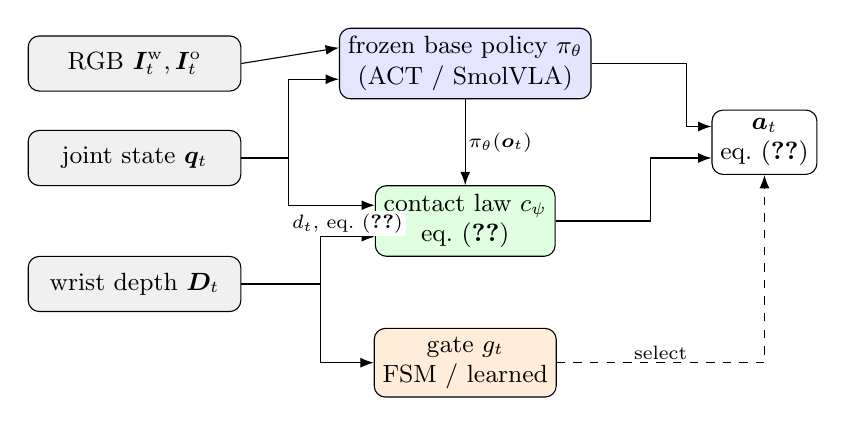
\begin{tikzpicture}[>=Latex,
  box/.style={draw,rounded corners,align=center,minimum height=7mm,inner sep=3pt,font=\small},
  sens/.style={box,fill=gray!12,minimum width=27mm},
  learn/.style={box,fill=blue!10},
  analytic/.style={box,fill=green!12},
  gatebox/.style={box,fill=orange!15},
  lab/.style={font=\scriptsize,fill=white,inner sep=1pt}]
% sensors (left column)
\node[sens] (rgb) at (0,2.2) {RGB $\img^{\mathrm{w}}_t,\img^{\mathrm{o}}_t$};
\node[sens] (q)   at (0,1.0) {joint state $\state_t$};
\node[sens] (d)   at (0,-0.6) {wrist depth $\depthmap_t$};
% processing (middle column)
\node[learn]    (pi) at (4.2,2.2) {frozen base policy $\pol$\\(ACT / SmolVLA)};
\node[analytic] (c)  at (4.2,0.2) {contact law $\ctrl$\\eq.~\eqref{eq:law}};
\node[gatebox]  (g)  at (4.2,-1.6) {gate $\gate_t$\\FSM / learned};
% mixer (right)
\node[box] (mix) at (8.0,1.2) {$\act_t$\\eq.~\eqref{eq:hybrid}};
% edges
\draw[->] (rgb.east) -- ([yshift=2mm]pi.west);
\draw[->] (q.east) -- ++(0.6,0) |- ([yshift=-2mm]pi.west);
\draw[->] (q.east) -- ++(0.6,0) |- ([yshift=2mm]c.west);
\draw[->] (d.east) -- ++(1.0,0) |- node[lab,pos=0.75,above]{$d_t$, eq.~\eqref{eq:roi}} ([yshift=-2mm]c.west);
\draw[->] (d.east) -- ++(1.0,0) |- (g.west);
\draw[->] (pi.south) -- node[lab,right]{$\pol(\obs_t)$} (c.north);
\draw[->] (pi.east) -- ++(1.2,0) |- ([yshift=2mm]mix.west);
\draw[->] (c.east) -- ++(1.2,0) |- ([yshift=-2mm]mix.west);
\draw[->,dashed] (g.east) -| node[lab,pos=0.25,above]{select} (mix.south);
\end{tikzpicture}}
\caption{Gated hybrid policy (\cref{def:hybrid}). Blue: learned; green: analytic; orange: the component this programme proposes to learn.}
\label{fig:arch}
\end{subfigure}\hfill
\begin{subfigure}[b]{0.40\textwidth}
\centering
\resizebox{\linewidth}{!}{%
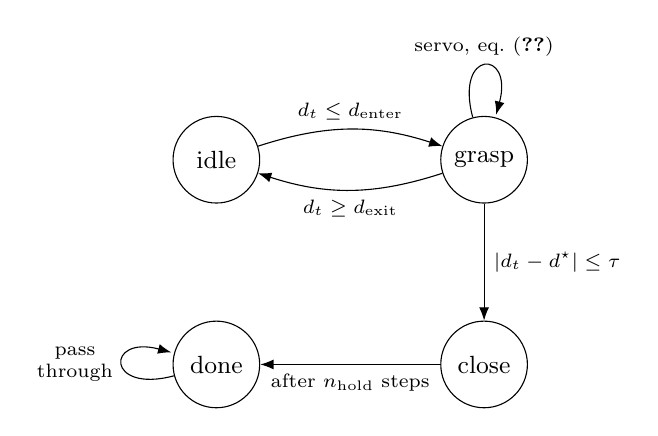
\begin{tikzpicture}[>=Latex,
  state/.style={draw,circle,minimum size=11mm,font=\small,inner sep=1pt},
  lab/.style={font=\scriptsize,align=center}]
\node[state] (idle) at (0,0) {idle};
\node[state] (gr)   at (3.4,0) {grasp};
\node[state] (cl)   at (3.4,-2.6) {close};
\node[state] (dn)   at (0,-2.6) {done};
\draw[->] (idle) to[bend left=18] node[lab,above]{$d_t\le d_{\mathrm{enter}}$} (gr);
\draw[->] (gr) to[bend left=18] node[lab,below]{$d_t\ge d_{\mathrm{exit}}$} (idle);
\draw[->] (gr) -- node[lab,right]{$|d_t-d^\star|\le\tau$} (cl);
\draw[->] (cl) -- node[lab,below]{after $n_{\mathrm{hold}}$ steps} (dn);
\draw[->] (gr) edge[loop above] node[lab]{servo, eq.~\eqref{eq:law}} (gr);
\draw[->] (dn) edge[loop left] node[lab,left]{pass\\through} (dn);
\end{tikzpicture}}
\caption{Threshold gate implemented in \texttt{DepthGraspController}.}
\label{fig:fsm}
\end{subfigure}
\caption{The hybrid policy as a switched system. The learned policy owns approach, transport and place; the analytic law owns the final descent and closure. The gate is the object of \cref{rq:gate}.}
\label{fig:hybrid}
\end{figure}

\subsection{Failure modes of the threshold gate}
\label{sec:chunk}

Two properties of \cref{eq:hybrid} with a threshold gate are not covered by prior work and motivate the learned-gate and chunk-aware variants.

\paragraph{False triggers.} The gate is a function of $d_t$ alone. Any object passing through $\mathcal{R}$ at a distance below $d_{\mathrm{enter}}$ during transport or place (the cup rim, the operator's hand) triggers the servo and may force closure. Gripper state, approach velocity $\dot d_t$ and the base policy's own intent (e.g. its predicted gripper trajectory over the chunk) are all available but unused.

\paragraph{Stale chunks.} The base policy executes a chunk planned at $t_0$ open-loop for up to $K$ steps. If the override moves the arm during $[t_{\mathrm{enter}},t_{\mathrm{exit}}]\subset[t_0,t_0+K]$, the remaining actions in the queue were planned for a trajectory the arm is no longer on (\cref{fig:chunk}). On release, the policy continues popping those actions until the queue drains, which can undo the correction or produce a discontinuity at the next replan. Temporal ensembling averages overlapping chunks and does not remove this; SmolVLA's asynchronous action queue has the same property. Candidate remedies are to flush the base policy's queue on phase exit, to blend rather than overwrite during a short hand-back window, or to learn the gate jointly with a replan signal.

\begin{figure}[t]
\centering
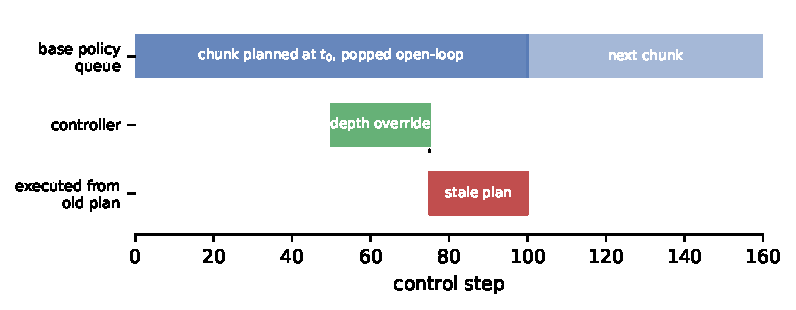
\includegraphics[width=0.78\textwidth]{chunk_override}
\caption{Interaction between an external override and open-loop action chunking. The chunk popped from $t_0$ remains in the queue after the override returns control at $t_{\mathrm{exit}}$; the red segment is executed from a plan made before the arm was moved.}
\label{fig:chunk}
\end{figure}

% ---------------------------------------------------------------------------
\section{Method: four uses of one depth stream}
\label{sec:method}

The same $\depthmap_t$ can enter the learning problem in four places. Each defines a policy family that the platform can already run or can run with a small extension; the hypotheses are stated so that the experiment in \cref{sec:design} can refute them.

\subsection{H1: depth as an analytic override}

The hybrid of \cref{def:hybrid} with the threshold gate and the law of \cref{eq:law}, wrapping a frozen ACT or SmolVLA. \Cref{alg:override} gives the per-step computation as implemented.

\begin{hypothesis}[contact proxy]\label{hyp:h1}
For a base policy whose failures are dominated by grasp instability, the depth-gated hybrid increases in-distribution success by at least 20 percentage points relative to the same frozen base, with the gain concentrated in trials whose failure class under the base policy is ``grasp instability''.
\end{hypothesis}

\begin{algorithm}[t]
\caption{Depth-gated override, one control step (as implemented in \texttt{depth\_grasp.py})}
\label{alg:override}
\begin{algorithmic}[1]
\Require base action $\act=\pol(\obs_t)$, state $\state_t$, depth map $\depthmap_t$, phase $s$, parameters $\psi=(\rho,d_{\mathrm{enter}},d^\star,d_{\mathrm{exit}},\tau,\kappa,\sigma,\Delta_{\max},n_{\mathrm{hold}})$
\State $d \gets$ ROI median of $\depthmap_t$ (\cref{eq:roi}); \textbf{if} $d$ undefined or $s=\textsc{done}$ \textbf{return} $\act$ \Comment{abstain}
\If{$s=\textsc{close}$} force gripper to $a^{\mathrm{closed}}$; decrement hold counter; $s\gets\textsc{done}$ when it reaches 0; \textbf{return} $\act$ \EndIf
\If{$s=\textsc{idle}$ \textbf{and} $d\le d_{\mathrm{enter}}$} $s\gets\textsc{grasp}$ \EndIf
\If{$s=\textsc{grasp}$ \textbf{and} $d\ge d_{\mathrm{exit}}$} $s\gets\textsc{idle}$; \textbf{return} $\act$ \EndIf
\If{$s=\textsc{grasp}$}
  \State $e\gets d-d^\star$
  \For{$j\in\mathcal{V}$} $\act_j \gets \state_{t,j} + \operatorname{clip}(\sigma_j\kappa e,-\Delta_{\max},\Delta_{\max})$ \EndFor
  \If{$|e|\le\tau$} $s\gets\textsc{close}$; start hold counter at $n_{\mathrm{hold}}$; force gripper closed \EndIf
\EndIf
\State \textbf{return} $\act$
\end{algorithmic}
\end{algorithm}

\subsection{H2: depth as an observation}

ACT is extended with a depth encoder $E_\omega:\R^{H\times W}\to\R^{h w\times d_{\mathrm{model}}}$, a three-layer strided CNN whose output is pooled to the RGB token grid and concatenated to the image tokens before the transformer encoder. The policy is trained end-to-end with \cref{eq:act} on RGB-D episodes. SmolVLA is not modified in the first phase; a PointVLA-style adapter that injects depth tokens into the frozen action expert~\citep{li2025pointvla} is the second-phase extension.

\begin{hypothesis}[input depth]\label{hyp:h2}
With tens of demonstrations and a from-scratch depth encoder, adding depth as an input does \emph{not} improve ACT's success in distribution and may reduce it, consistent with~\citep{ze2024dp3}; any benefit appears only in out-of-distribution height conditions.
\end{hypothesis}

\subsection{H3: depth as a teacher (override-as-DAgger)}
\label{sec:distill}

Every hybrid rollout yields pairs $(\obs_t,\act^{\mathrm{h}}_t)$ in which the contact-phase actions were produced by the analytic law from metric depth. Following DAgger~\citep{ross2011dagger} with the controller as the expert during gated steps only, we aggregate
\begin{equation}
\mathcal{D}_{k+1} = \mathcal{D}_k \;\cup\; \big\{(\obs_t,\act^{\mathrm{h}}_t) : \gate_t=1,\; \text{rollout } \in \text{iteration } k\big\},
\label{eq:dagger}
\end{equation}
and retrain an \emph{RGB-only} ACT on $\mathcal{D}_{k+1}$. The resulting policy sees no depth at test time; the geometric information has been distilled into its visual features, in the spirit of SPARTN~\citep{zhou2023spartn} but with corrections generated by a sensor rather than by novel-view synthesis.

\begin{hypothesis}[distillation]\label{hyp:h3}
After one or two aggregation rounds, the RGB-only policy trained on $\mathcal{D}_{k}$ recovers a majority of the hybrid's in-distribution gain without the sensor, but less of its out-of-distribution gain.
\end{hypothesis}

\subsection{H4: a learned gate}
\label{sec:gate}

Replace the threshold automaton by $\gate_t = \ind[\sigma(f_\phi(\bm{x}_t)) > 0.5]$ with features
\begin{equation}
\bm{x}_t = \big(d_t,\;\dot d_t,\;\nu_t,\;\state_t,\;\hat{\act}^{\mathrm{grip}}_{t:t+K}\big),
\end{equation}
where $\nu_t$ is the valid-pixel fraction of the ROI and the last term is the base policy's predicted gripper trajectory over its current chunk (a cheap read of intent). Phase labels are recovered from existing demonstrations without new annotation: the closure onset $t_c$ in each episode is the first step at which the leader gripper command drops below the closed threshold, and the contact phase is labelled $[t_c-\Delta_{\mathrm{pre}},\,t_c+\Delta_{\mathrm{post}}]$. $f_\phi$ is a small MLP or GRU trained with class-weighted cross-entropy, with a hysteresis post-filter to prevent chatter.

\begin{hypothesis}[learned gate]\label{hyp:h4}
The learned gate reduces false-trigger events per trial and stale-chunk discontinuities relative to the threshold gate at equal or higher task success, and is more robust to $d_{\mathrm{enter}}$ mis-specification (the threshold gate degrades monotonically as $d_{\mathrm{enter}}$ moves away from its tuned value).
\end{hypothesis}

\subsection{Chunk-aware hand-back}
Orthogonal to H1--H4, two hand-back rules are compared within the hybrid: (a) \emph{overwrite} (current), (b) \emph{flush}, which empties the base policy's action queue on \textsc{grasp}$\to$\textsc{idle} and \textsc{close}$\to$\textsc{done} so that the next base action is replanned from the corrected state, and (c) \emph{blend}, $\act_t = \lambda_t\pol(\obs_t) + (1-\lambda_t)\ctrl(\cdot)$ with $\lambda_t$ ramping from 0 to 1 over a short window. Flush is a two-line change to the policy interface and is the default for all H1--H4 arms unless it is shown to hurt.

% ---------------------------------------------------------------------------
\section{Experimental design}
\label{sec:design}

\subsection{Platform and task}

\begin{figure}[t]
\centering
\begin{subfigure}[b]{0.36\textwidth}
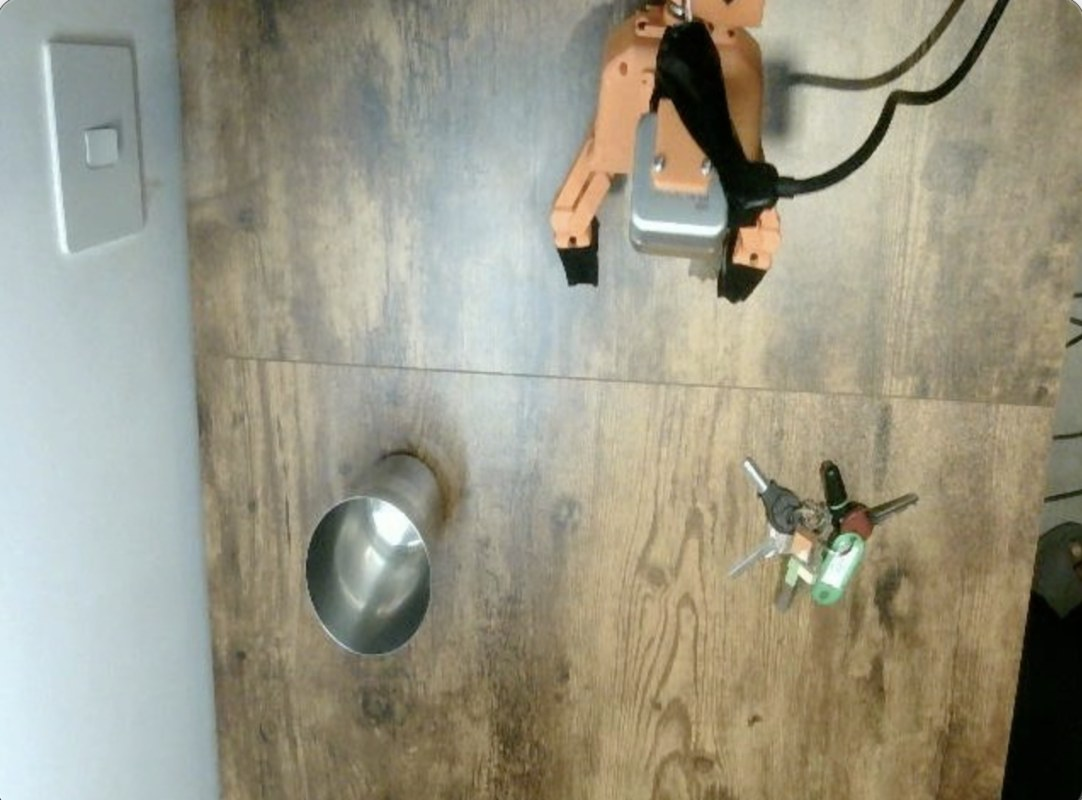
\includegraphics[width=\textwidth]{overhead_real}
\caption{Overhead view: follower gripper, metal cup, key ring.}
\end{subfigure}\hfill
\begin{subfigure}[b]{0.36\textwidth}
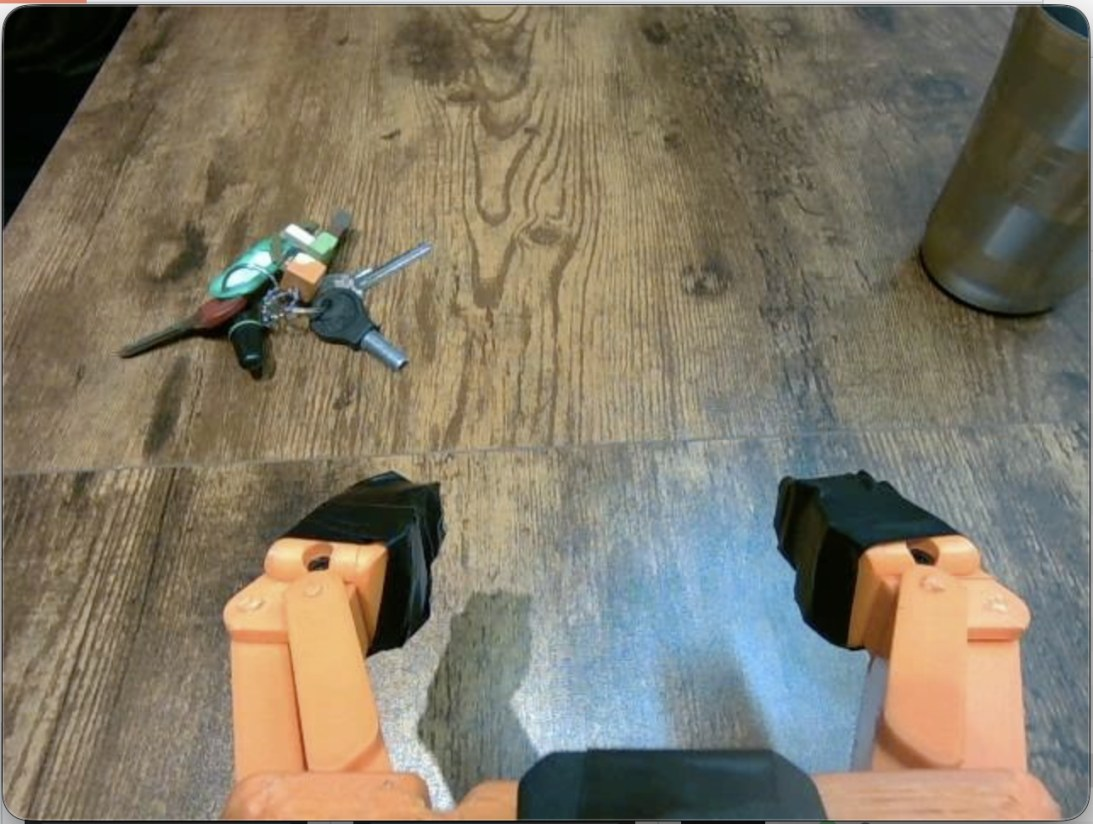
\includegraphics[width=\textwidth]{wrist_real}
\caption{Wrist (eye-in-hand) RGB.}
\end{subfigure}\hfill
\begin{subfigure}[b]{0.25\textwidth}
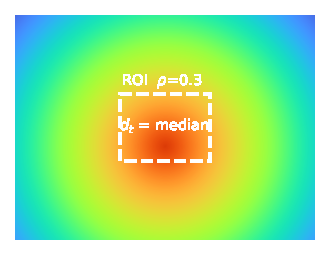
\includegraphics[width=\textwidth]{roi_overlay}
\caption{Wrist depth with the controller's ROI (illustrative rendering).}
\end{subfigure}
\caption{Observation modalities on the SO-101 cell. (a) and (b) are real frames from the cell; (c) is the repository's placeholder depth rendering, used here only to show the ROI geometry. The ROI median of the real D405 frame is the scalar $d_t$ in \cref{eq:roi}.}
\label{fig:views}
\end{figure}

The cell is a pair of SO-101 arms (leader for teleoperation, follower as the plant), six STS3215 servos per arm at 12\,V, an Intel RealSense D405 on the follower wrist (RGB and metric depth, aligned), and a USB overhead RGB camera. Sensing runs on a separate Windows node and is streamed over ZMQ; control, training and evaluation run on a Mac (\cref{fig:views}). The task is ``place keys into the metal cup''. Success requires the keys inside the cup, the gripper clear of the keys, and nothing knocked over; the criterion is frozen in the protocol file before any evaluation.

\subsection{Factors and conditions}

\begin{table}[t]
\centering\small
\caption{Pre-registered experiment matrix. Each row is run under identical protocol, cameras, task string and operator script. ID: three key positions. OOD: table height $\pm$2\,cm via a riser, a larger/smaller key ring, and two distractor objects. Minimum trials per row and split are set by the power analysis in \cref{sec:stats}.}
\label{tab:matrix}
\begin{tabularx}{\textwidth}{@{}l l l X@{}}
\toprule
Row & Base policy & Depth use & Hypothesis / purpose \\
\midrule
A1 & ACT & none & baseline \\
A2 & ACT & input tokens & H2 \\
A3 & ACT + hybrid (threshold gate) & override & H1 \\
A4 & ACT + hybrid (learned gate) & override & H4 \\
A5 & ACT retrained on $\mathcal{D}_1$, RGB-only & distilled & H3 \\
S1 & SmolVLA & none & baseline \\
S2 & SmolVLA + hybrid (threshold gate) & override & H1 (VLA base) \\
S3 & SmolVLA + hybrid (learned gate) & override & H4 (VLA base) \\
\bottomrule
\end{tabularx}
\vspace{2pt}
\begin{flushleft}\footnotesize
Within-row sub-factors (counter-balanced): hand-back rule $\in\{$overwrite, flush$\}$ for all hybrid rows; $d_{\mathrm{enter}}\in\{150,180,220\}$\,mm sensitivity sweep for A3 and S2 only.
\end{flushleft}
\end{table}

\Cref{tab:matrix} lists the arms. Rows are evaluated in \emph{interleaved} order (A1, A3, S1, S2, \dots within each session) so that drift in lighting, battery and operator behaviour is not confounded with policy. The scorer is given the trial outcome without being told which row produced it wherever the robot's motion does not reveal it.

\subsection{Metrics}

Per trial we record: binary success $Y$; a primary failure class from the taxonomy of~\citep{yu2026so101} (grasp instability, repetition loop, state mismatch, precision misalignment) plus ``false trigger'' and ``stale chunk'' for hybrid rows; recovery opportunities and successes; time to first closure; steps to termination; and, for hybrid rows, the depth error at closure $e_{t_c}=d_{t_c}-d^\star$, which is the only direct measurement of grasp-height error available on this platform. Overall and per-condition success rates are reported with counts, never as percentages alone.

\subsection{Statistical analysis and power}
\label{sec:stats}

Success rates are reported with 95\% Wilson intervals~\citep{wilson1927}. Pairwise comparisons between a hybrid row and its base use a two-sided Fisher exact test on the pooled ID trials and a Beta-Binomial posterior $P(p_{\mathrm{hyb}}>p_{\mathrm{base}}\mid\text{data})$ with uniform priors. To limit trial cost, comparisons are run as a sequential test~\citep{snyder2025comparison} with a cap, so that a clear effect stops early without inflating the false-positive rate.

\begin{figure}[t]
\centering
\begin{subfigure}[b]{0.48\textwidth}
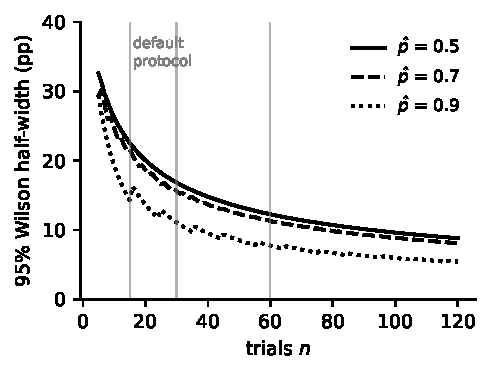
\includegraphics[width=\textwidth]{ci_width}
\caption{Interval half-width versus trials.}
\label{fig:ci}
\end{subfigure}\hfill
\begin{subfigure}[b]{0.48\textwidth}
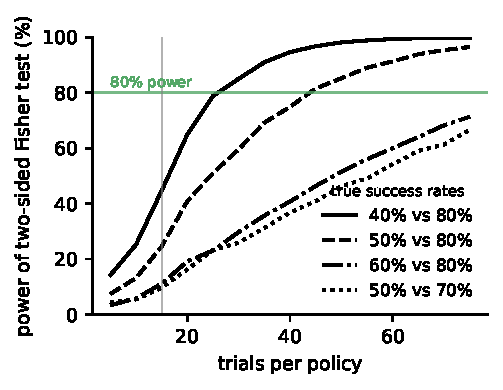
\includegraphics[width=\textwidth]{power}
\caption{Power of a two-sided Fisher test at $\alpha=0.05$.}
\label{fig:power}
\end{subfigure}
\caption{Why the default budget is insufficient. The platform's default protocol (vertical line, 15 trials) yields $\pm$20-point intervals and under 50\% power even for a 40-point effect; 30 trials per policy reach 80\% power for a 40-point effect but remain underpowered for a 20-point effect.}
\label{fig:stats}
\end{figure}

\Cref{fig:stats} quantifies the budget. With 15 trials an observed 10/15 has interval $[42\%,85\%]$; a per-condition 3/5 has $[23\%,88\%]$. With 15 trials per policy the Fisher test has 45\% power for a 40\% vs 80\% difference and 10\% for 60\% vs 80\%. We therefore pre-register \textbf{a minimum of 30 ID trials per row} (10 per key position), a sequential cap of 60, and treat 20-point effects as exploratory unless the sequential test terminates. OOD conditions are analysed as a secondary endpoint with the same machinery.

\subsection{Threats to validity}
\emph{Internal.} Operator reset variability is controlled by taped marks and photographed initial conditions; scorer bias by the blinding described above; threshold tuning leakage by fixing $\psi$ on a separate tuning set of ten rollouts before any scored trial. \emph{Construct.} Binary success hides contact-phase behaviour; the failure taxonomy and $e_{t_c}$ address this. \emph{External.} One cell, one task; results are claims about the SO-101 class and this task family, and the cross-platform question is explicitly out of scope for this programme.

% ---------------------------------------------------------------------------
\section{Pilot analysis on fixture data}
\label{sec:pilot}

\textbf{The numbers in this section are illustrative fixtures shipped with the repository to exercise the reporting pipeline; they are not measurements.} They are included because they show, on exactly the shape of data the protocol produces, what the analysis of \cref{sec:stats} will and will not be able to conclude.

\begin{figure}[t]
\centering
\begin{subfigure}[b]{0.6\textwidth}
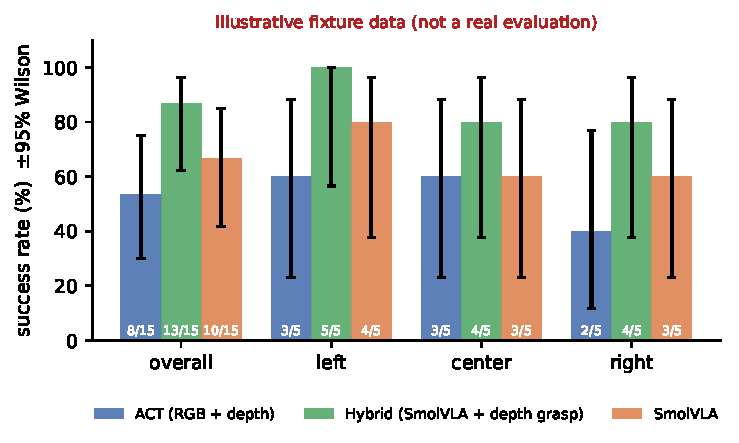
\includegraphics[width=\textwidth]{success_with_ci}
\caption{Overall and per-condition rates with 95\% Wilson intervals.}
\label{fig:pilot-ci}
\end{subfigure}\hfill
\begin{subfigure}[b]{0.38\textwidth}
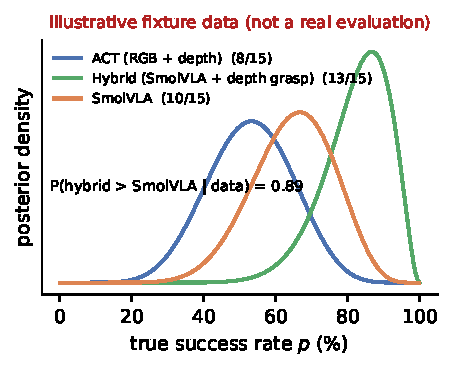
\includegraphics[width=\textwidth]{posteriors}
\caption{Beta posteriors over the true success rate.}
\label{fig:pilot-post}
\end{subfigure}
\caption{Analysis pipeline applied to the repository's fixture summaries (15 trials per method). Even a nominal 20-point gap between SmolVLA and the hybrid yields $P(\text{hybrid}>\text{SmolVLA})\approx0.89$ and overlapping intervals; a real evaluation at this budget could not support the claim.}
\label{fig:pilot}
\end{figure}

\Cref{fig:pilot} applies the reporting pipeline to the three fixture summaries (ACT with depth 8/15, SmolVLA 10/15, hybrid 13/15). The overall intervals overlap substantially and the posterior probability that the hybrid is better than SmolVLA is 0.89, short of any conventional threshold; the per-condition intervals span more than 60 points. This is the quantitative reason \cref{sec:stats} raises the trial budget.

\begin{figure}[t]
\centering
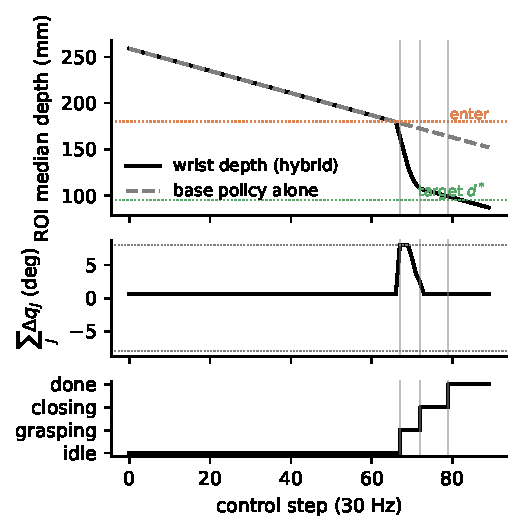
\includegraphics[width=0.55\textwidth]{controller_response}
\caption{Closed-loop response of the implemented contact law (\cref{alg:override}) driven against a one-dimensional plant in which the base policy descends toward a height 20\,mm too high. Dashed: base policy alone stalls above $d^\star$. Solid: the hybrid takes control at $d_{\mathrm{enter}}$, servos to $d^\star$ under the rate limit $\Delta_{\max}$, and forces closure. Produced by \texttt{research/scripts/make\_figures.py} using the repository's controller class.}
\label{fig:ctrl}
\end{figure}

\Cref{fig:ctrl} verifies that the implemented law behaves as \cref{eq:law} specifies: proportional descent saturating at the rate limit, convergence to within $\tau$ of $d^\star$, and a timed closure. It also exposes the parameters a learned gate must not depend on: the entry threshold determines \emph{when} the correction starts but not whether it converges.

% ---------------------------------------------------------------------------
\section{Research plan}
\label{sec:plan}

The programme is organised as five phases, each gated by a deliverable rather than a date.

\begin{enumerate}[leftmargin=*,itemsep=3pt]
\item \textbf{Instrumentation.} Add per-trial failure class, recovery events, time-to-closure and $e_{t_c}$ to the protocol logger; add Wilson intervals, Fisher/Beta comparison and a sequential-test stopping rule to the summary; add the \emph{flush} hand-back and an OOD condition set to the protocol YAML. Deliverable: a dry run of \cref{tab:matrix} rows A1 and A3 at 10 trials each with complete logs.
\item \textbf{H1 and H2.} Record the demonstration corpus with depth; train A1, A2 and the SmolVLA fine-tune; run A1--A3 and S1--S2 to the pre-registered budget with interleaving and blinding. Deliverable: the first controlled answer to \cref{rq:proxy} and the in-distribution half of \cref{rq:where}.
\item \textbf{H3.} Collect $\mathcal{D}_1$ from the A3 rollouts; retrain RGB-only ACT; run A5. Deliverable: whether depth can be removed at test time (\cref{rq:where}).
\item \textbf{H4.} Extract closure-onset labels from the corpus; train $f_\phi$; run A4 and S3, plus the $d_{\mathrm{enter}}$ sensitivity sweep on A3/S2. Deliverable: \cref{rq:gate}.
\item \textbf{OOD and synthesis.} Run the OOD split for every row that survived phase 2--4; analyse the ID--OOD interaction. Deliverable: \cref{rq:ood} and the final comparison across the four depth uses.
\end{enumerate}

\paragraph{Risks.}
(i) The D405 returns invalid depth on the reflective cup and on thin key rings; mitigation is the abstention branch of \cref{alg:override} and the valid-fraction feature of the learned gate, and a fallback to a matte target set. (ii) Servo backlash makes $\state_t$ an inaccurate proxy for fingertip pose; this affects all arms equally and is part of what ``force-blind, low-cost'' means. (iii) Human trial throughput bounds the budget at roughly 60--80 scored trials per session; the sequential test and interleaving are designed around this.

% ---------------------------------------------------------------------------
\section{Discussion and expected impact}

If \cref{hyp:h1} holds and \cref{hyp:h2} holds as stated, the conclusion is that for small-data imitation learning on force-blind hardware, geometric information is best applied \emph{outside} the network, in the controller, and the common practice of concatenating a depth channel is not merely unhelpful but a source of variance. If \cref{hyp:h3} then holds, the controller's role becomes transitional: it is a teacher that makes the RGB policy contact-aware, after which the sensor can be removed, which matters for cost-constrained deployments. If \cref{hyp:h4} holds, the learned-coarse / analytic-fine pattern becomes a general recipe in which only the hand-off is learned, a far smaller learning problem than residual RL and one that needs neither force sensing nor a simulator. A negative result on \cref{hyp:h1} would be equally informative: it would indicate that grasp instability on this embodiment is dominated by lateral error or by closure timing rather than by height, redirecting effort toward lateral servoing on the wrist image or toward closure prediction.

Beyond the specific hypotheses, the programme contributes an evaluation standard for single-cell low-cost robotics: pre-registered matrices, powered budgets, interleaved and blinded scoring, failure attribution, and sequential stopping, all implemented in a protocol file that travels with the code.

% ---------------------------------------------------------------------------
\section{Conclusion}

We have cast the depth-assisted hybrid grasp of the SO-101 platform as a machine-learning research programme rather than a pipeline feature. The central object is a gated switched policy in which metric wrist depth stands in for the force feedback the embodiment lacks; the central question is where in the learning problem that depth should enter. The formulation yields four falsifiable hypotheses, an identified and remediable interaction with action chunking, a learned-gate extension whose labels come for free from existing demonstrations, and a powered, pre-registered real-robot protocol. The platform already implements the baseline and the override; the remaining work is measurement.

% ---------------------------------------------------------------------------
\bibliographystyle{plainnat}
\bibliography{references}

% ---------------------------------------------------------------------------
\appendix
\section{Notation}
\begin{table}[h]
\centering\small
\begin{tabular}{@{}ll@{}}
\toprule
Symbol & Meaning \\
\midrule
$\obs_t,\act_t,\state_t$ & observation, joint-target action, joint state at step $t$ \\
$\img^{\mathrm{w}}_t,\img^{\mathrm{o}}_t,\depthmap_t$ & wrist RGB, overhead RGB, wrist metric depth (mm) \\
$\pol$ & frozen base policy (ACT or SmolVLA) \\
$\ctrl$ & analytic contact law with parameters $\psi$ \\
$\gate_t, s_t$ & gate and discrete phase \\
$d_t, d^\star, e_t$ & ROI median depth, target depth at closure, depth error \\
$z_t, z^\star, \delta_{\mathrm{cam}}$ & fingertip height, closure height, camera-to-fingertip offset \\
$\kappa,\sigma_j,\Delta_{\max},\tau$ & servo gain, joint sign, per-step rate limit, closure tolerance \\
$d_{\mathrm{enter}},d_{\mathrm{exit}},n_{\mathrm{hold}}$ & gate thresholds and closure hold length \\
$K,n_a$ & chunk length and executed prefix length \\
$\mathcal{D}_k$ & aggregated dataset after $k$ override-as-teacher rounds \\
\bottomrule
\end{tabular}
\end{table}

\section{Controller parameters as shipped}
\begin{table}[h]
\centering\small
\caption{Default values in \texttt{config/hybrid\_grasp.yaml}. Units: mm, deg.}
\begin{tabular}{@{}lrl@{}}
\toprule
Parameter & Value & Role \\
\midrule
\texttt{roi\_frac} ($\rho$) & 0.30 & centred ROI fraction for \cref{eq:roi} \\
\texttt{enter\_mm} ($d_{\mathrm{enter}}$) & 180 & take control \\
\texttt{target\_mm} ($d^\star$) & 95 & servo set-point \\
\texttt{exit\_mm} ($d_{\mathrm{exit}}$) & 280 & release control \\
\texttt{tol\_mm} ($\tau$) & 15 & closure band \\
\texttt{min\_mm}, \texttt{max\_mm} & 40, 2000 & valid depth range \\
\texttt{gain\_deg\_per\_mm} ($\kappa$) & 0.08 & proportional gain \\
\texttt{max\_delta\_deg} ($\Delta_{\max}$) & 4.0 & per-step rate limit per joint \\
\texttt{vertical\_joints} ($\mathcal{V}$) & lift, elbow & joints the law moves \\
\texttt{gripper\_closed}, \texttt{hold\_close\_frames} & 15, 8 & closure value and hold length \\
\bottomrule
\end{tabular}
\end{table}

\section{Evaluation protocol file}
\begin{verbatim}
task: Place keys into metal cup
timeout_s: 60
n_trials_per_condition: 5        # pre-registered minimum: 10 (30 ID trials)
success_criterion: >
  Keys are inside the metal cup, gripper is clear of the keys, and nothing was
  knocked over.
conditions:
  - {id: keys=left,   pen: left,   distractors: none, split: id}
  - {id: keys=center, pen: center, distractors: none, split: id}
  - {id: keys=right,  pen: right,  distractors: none, split: id}
  # OOD rows added in phase 1 of the research plan:
  # - {id: height+2cm,  pen: center, split: ood}
  # - {id: ring-large,  pen: center, split: ood}
  # - {id: distractors, pen: center, distractors: two, split: ood}
\end{verbatim}

\end{document}
